\documentclass[a4paper,10pt]{article}
%-----------------------------------------------------------
\usepackage[top=0.75in, bottom=0.75in, left=0.55in, right=0.85in]{geometry}
\usepackage{graphicx}
\usepackage{url}
\usepackage{palatino}
\usepackage{tabularx}
\fontfamily{Calibri}
\selectfont

\usepackage[T1]{fontenc}
\usepackage
%[ansinew]
[utf8]
{inputenc}

\usepackage{color}
\definecolor{mygrey}{gray}{0.75}
\textheight=9.75in
\raggedbottom

\setlength{\tabcolsep}{0in}
\newcommand{\isep}{-2 pt}
\newcommand{\lsep}{-0.5cm}
\newcommand{\psep}{-0.6cm}
\renewcommand{\labelitemii}{$\circ$}

\pagestyle{empty}
%------------------------------------------------------------
%Custom commands
\newcommand{\resitem}[1]{\item #1 \vspace{-2pt}}
\newcommand{\resheading}[1]{{\small \colorbox{mygrey}{\begin{minipage}{0.975\textwidth}{\textbf{#1 \vphantom{p\^{E}}}}\end{minipage}}}}
\newcommand{\ressubheading}[3]{
\begin{tabular*}{6.62in}{l @{\extracolsep{\fill}} r}
	\textsc{{\textbf{#1}}} & \textsc{\textit{[#2]}} \\
\end{tabular*}\vspace{-8pt}}
%-----------------------------------------------------------

\begin{document}
\hspace{0.5cm}\\[-0.2cm]
\begin{flushright}
\large
\textbf{Niharika Jayanthi} \\
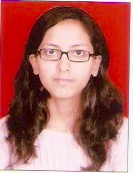
\includegraphics[width = 30mm]{NJ.jpeg}
\end{flushright}

\indent \resheading{\textbf{CONTACT INFORMATION} }\\[\lsep]
\\ \\

\indent\begin{tabular}{@{}p{3.5in}p{3.5in}}
23/A HP Nagar East, &  {Phone No.:} +91 9167073228 \\ 
Chembur, Vashinaka,	&  {Email-id:} niharika\_jayanthi@yahoo.co.in \\
Mumbai- 400074   \\
\end{tabular}

\indent\resheading{\textbf{CAREER OBJECTIVE} }\\[\lsep]
\\ \\
\indent To work in a challenging environment that provides generous opportunities for personal and professional \indent development.

\indent\resheading{\textbf{EDUCATION} }\\[\lsep]
\\ \\
\indent \begin{tabular}{ l @{\hskip 0.15in} l @{\hskip 0.15in} l @{\hskip 0.15in} l @{\hskip 0.15in} l}
	\hline
	\textbf{Examination} & \textbf{University} & \textbf{Institute} & \textbf{Year} & \textbf{CPI} \\
	\hline
	10th Board & CBSE & St. Anselm Senior Secondary School, Jaipur & 2010 & 9.6 \\
	\hline
	12th Board & CBSE & Delhi Public School, Navi Mumbai & 2012 & 86\% \\
	\hline
	B.E. & Mumbai University & Fr. C. Rodrigues Institute of Technology, Vashi & 2016 & 7.35\\
	\hline
\end{tabular}
\\ \\

\resheading{\textbf{PROJECTS} }\\[\lsep]
\\ \\
\begin{enumerate}
	\item SYLLABUS COVERAGE TIMELINE GENERATOR
	\subitem This project automated a teacher's task of manually drawing a timeline for their syllabus coverage. The front-end was written in Python. The back-end used SQL Lite 3 database.
	\item EXCEL IMPORTER AND EXPORTER
	\subitem This project enabled easy importing and exporting of an excel database from and to a MySQL database while maintaining the integrity of both. The front-end was developed using Python.
\end{enumerate}


\resheading{\textbf{TRAINING AND INTERNSHIP} }\\[\lsep]
\\ \\
\begin{itemize}
	\item Python:
	Attended a Python workshop conducted by college under CSI.
	\item No internships yet.
\end{itemize}

\resheading{\textbf{RESEARCH PUBLICATIONS} }\\[\lsep]
\\ \\
\begin{enumerate}
	\item No research publications yet.
\end{enumerate}


\resheading{\textbf{TECHNICAL SKILLS} }\\[\lsep]
\\ \\
\begin{itemize}
	\item \noindent \textbf{Languages} (C, C++, Python, Java)
	\item \noindent \textbf{Database} (MySQL, Microsoft SQL Server)
	\item \noindent \textbf{Script} (HTMl, CSS, Javascript).
\end{itemize}


\resheading{\textbf{SOFT SKILLS} }\\[\lsep]
\\ \\
\begin{enumerate}
	\item \noindent Strong verbal and written communication skills.
	\item \noindent Managed strict project timelines through efficient planning and coordination among team members.
	\item \noindent Adapted with respect to changing deadlines by re-evaluating priorites.
	\item \noindent Initiated and led brainstorming sessions for process improvement.
	\item \noindent Resolved conflicts among team members with quick and effective communication.
\end{enumerate}

\resheading{\textbf{EXTRA CURRICULAR ACTIVITIES} }\\[\lsep]
\\ \\
\begin{itemize}
	\item Won food fest competition, a team event, in 2014.
	\item Came first in relay race in 2012.
	\item Came second in table tennis girls' doubles, a college-level competition.
	\item Participated in face-painting competition.
\end{itemize}


\resheading{\textbf{CO-CURRICULAR ACTIVITIES} }\\[\lsep]
\\ \\
\begin{enumerate}
	\item \noindent Conducted a workshop 'Python for Beginners' under Cryptex-2014.
	\item \noindent Came first in Cryptex coding competition conducted under CSI.
	\item \noindent Participated in CodeVita, coding competition conducted by TCS.
	\item \noindent Took part in e-YRC in the years 2013 and 2014.
	
\end{enumerate}

\resheading{\textbf{PERSONAL INFORMATION} }\\[\lsep]
\\ \\
\indent Father’s Name: J. S. Prasad \\
\indent Mother’s Name: J. L. Umabala \\
\indent Sex: Female \\
\indent Date of Birth: May 6, 1994 \\
\indent Nationality: Indian \\
\indent Marital Status: Single \\

\resheading{\textbf{REFERENCE} }\\[\lsep]
\\ \\

\resheading{\textbf{DECLARATION} }\\[\lsep]
\\ \\

\resheading{\textbf{DATE} }\\[\lsep]
\\ \\

\end{document}

